\chapter{Work Breakdown Structure}
\label{chpt:WBS}

The Work Breakdown Structure (WBS) provides a hierarchical decomposition of all
mission-related tasks and system elements. It ensures full traceability of responsibilities, technical
components, and documentation deliverables across the project lifecycle. 

This document presents the initial version of the WBS. It serves as a foundation for current planning
and coordination, but it is expected to evolve during subsequent design, integration, and operations
phases. Additional branches and refinements may be incorporated.

\section{Purpose and Role of the WBS}

The WBS is a hierarchical framework that organizes the total scope
of the mission into manageable elements. It supports key project management activities, including:
\begin{itemize}
    \item Definition of scope and deliverables
    \item Assignment of responsibilities
    \item Scheduling and resource allocation
    \item Risk identification and mitigation
    \item Cost estimation and progress tracinkg    
\end{itemize}

By breaking the mission, as a complicated project, down into functionally and logically grouped components, the WBS enables consistent communication between stakeholders, ensures no aspect of the mission is overlooked, and provides a roadmap for technical and managerial execution.

\section{Structural Logic and Content Overview} 
The WBS is structured into six top-level categories (Level1), each representing a distinct phase or domain of the mission. Each is further subdivided into lower-level elements that reflect the major systems, subsystems, and work packages necessary for
mission success. The current WBS emphasizes clarity and modularity, aligning with the project's scale and technology-demonstration character.
\begin{enumerate}
    \item \textbf{Project Management} – Encompasses the administrative coordination and organizational backbone
    \item \textbf{Mission Definition and Analysis} – Captures the conceptual and feasibility phases of the project. It defines the mission purpose, scientific and technological objectives (centred on the perovskite payload), and outlines the required data products and user scenarios.
    \item \textbf{System Engineering} – Covers the technical design and integration of both the space and ground segments. It includes the engineering of all onboard subsystems (EPS, AOCS, OBDHS, etc.), the payload, and the operational infrastructure on the ground. Dedicated nodes ensure that system interfaces and resource budgets are carefully defined and monitored.
    \item \textbf{Assembly, Integration, and Testing (AIT)} – Details the integration processes and verification protocols that will be used to assemble the flight model, validate subsystem performance, and ensure compatibility with the launch environment.
    \item \textbf{Launch} – Describes planning and execution of launch-related activities, from launcher selection and mechanical interfacing to campaign logistics and operational readiness.
    \item \textbf{Mission Operation} – Defines post-launch operational activities, including commissioning, routine functioning, anomaly resolution, timeline management, and end-of-life strategies.
\end{enumerate}

 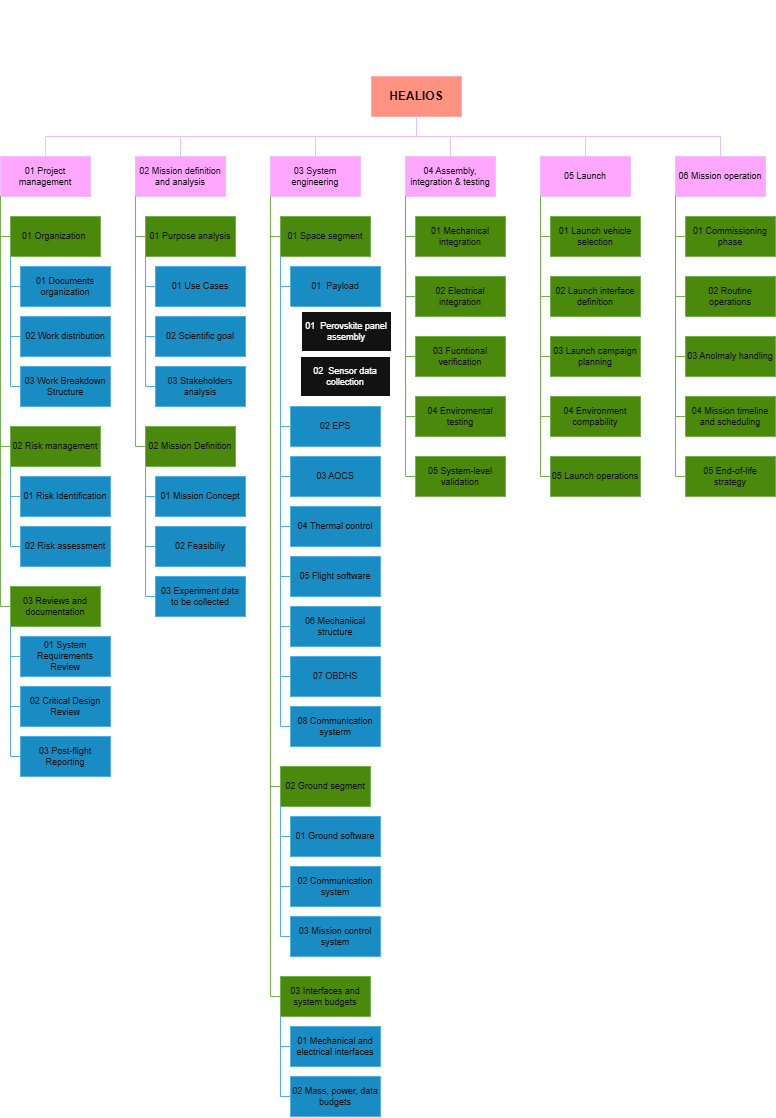
\includegraphics[width=\textwidth, keepaspectratio]{figures/01_01_03_Initial_WBS.png}
